\documentclass[letterpaper]{article}
\usepackage[utf8]{inputenc}
\usepackage[T1]{fontenc}
\usepackage[activeacute,english]{babel}
\usepackage[vmargin=4cm,tmargin=3cm,hmargin=2cm,letterpaper]{geometry}%
\usepackage{helvet}
\usepackage{amsmath,amsfonts,amssymb}
\usepackage{graphicx}
\usepackage{color}
\usepackage{xcolor}
\usepackage{verbatim}
\usepackage{tabls}
\usepackage{lastpage}
\usepackage{fancyhdr}
\usepackage{url}
\usepackage{listings}
\usepackage{tikz}
\usepackage{pgf}
\usepackage{pgffor}
\usepgfmodule{plot}
\usepackage{wrapfig}
\usepackage{ifpdf}
\usepackage{amssymb}
\usepackage{pifont}
\usepackage{epstopdf}
\usepackage{graphicx} % Allows including images
\usepackage{booktabs} % Allows the use of \toprule, \midrule and \bottomrule in tables
\usepackage{tikz}
\usetikzlibrary{arrows,decorations,snakes,backgrounds,fit,calc,through,scopes,positioning,automata,chains,er,fadings,calendar,matrix,mindmap,folding,patterns,petri,plothandlers,plotmarks,shadows,shapes,shapes.arrows,topaths,trees}

\lstset{% general command to set parameter(s)
%   basicstyle=\small,
  % print whole listing small
%   keywordstyle=\color{black}\bfseries\underbar,
  % underlined bold black keywords
%   identifierstyle=,
  % nothing happens
%   commentstyle=\color{white}, % white comments
%   stringstyle=\ttfamily,
  % typewriter type for strings
  showstringspaces=false}
  % no special string spaces

\pagestyle{fancy}
\color{black}
\fancyhead{}
\renewcommand{\headrule}{\hrule\vspace*{0.5mm}\rule{\linewidth}{0.8mm}}
\renewcommand{\familydefault}{\sfdefault}

\graphicspath{{./images/}}
\lhead{
\includegraphics[width=2cm]{logoucr.png}}
\rhead{
\includegraphics[width=3cm]{eie-text-gray-6x3cm.png}}
\chead{UNIVERSIDAD DE COSTA RICA\\FACULTAD DE INGENIERÍA\\ESCUELA DE INGENIERÍA ELÉCTRICA\\\textbf{ESTRUCTURAS ABSTRACTAS DE DATOS Y\\ ALGORITMOS PARA INGENIERÍA}\\IE-0217\\I CICLO 2014\\PROPUESTA DEL PROYECTO DE ESTRUCTURAS DE DATOS}

\lfoot{}%
\cfoot{}%
%\cfoot{\thepage\ de \pageref{LastPage}}%
\rfoot{}%

%%%%%%%%%%%%%%%%%%%%%%%%%%%%%%%%%%%%%%%%%%%%%%%%%%%%%%%%%%%%%%%%%%%%%%%%%%%%%%%%%%%%%%%%%%%%%%%%%%%%%%%%%%%%%%%
\newcommand{\uic}{blue} %user-input color
%%%%%%%%%%%%%%%%%%%%%%%%%%%%%%%%%%%%%%%%%%%%%%%%%%%%%%%%%%%%%%%%%%%%%%%%%%%%%%%%%%%%%%%%%%%%%%%%%%%%%%%%%%%%%%%%%%
\newcommand{\uim}{\_\_} %user-input marker
%%%%%%%%%%%%%%%%%%%%%%%%%%%%%%%%%%%%%%%%%%%%%%%%%%%%%%%%%%%%%%%%%%%%%%%%%%%%%%%%%%%%%%%%%%%%%%%%%%%%%%%%%%%%%%%%%%
\newcommand{\userinput}[1]{\textcolor{\uic}{\uim#1\uim}}


%%%%%%%%%%%%%%%%%%%%%%%%%%%%%%%%%%%%%%%%%%%%%%%%%%%%%%%%%%%%%%%%%%%%%%%%%%%%%%%%%%%%%%%%%%%%%%%%%%%%%%%%%%%%%%%%%%
\begin{document}\vspace*{2cm}
%%%%%%%%%%%%%%%%%%%%%%%%%%%%%%%%%%%%%%%%%%%%%%%%%%%%%%%%%%%%%%%%%%%%%%%%%%%%%%%%%%%%%%%%%%%%%%%%%%%%%%%%%%%%%%%%%%

%%%%%%%%%%%%%%%%%%%%%%%%%%%%%%%%%%%%%%%%%%%%%%%%%%%%%%%%%%%%%%%%%%%%%%%%%%%%%%%%%%%%%%%%%%%%%%%%%%%%%%%%%%%%%%%%%%
\begin{center}
\Huge
\textbf{Data Structures Implementations for K-Da Library}
\vspace*{1cm}
\end{center}

\noindent
\small\baselineskip=14pt
\textbf{Estudiantes:} \\
\text{David Pérez Bolaños - B04769}\\
\text{Andrey Pérez Salazar - B25084}\\
\text{Andrés Sánchez López - B26214}\\


\begin{figure}[ht]
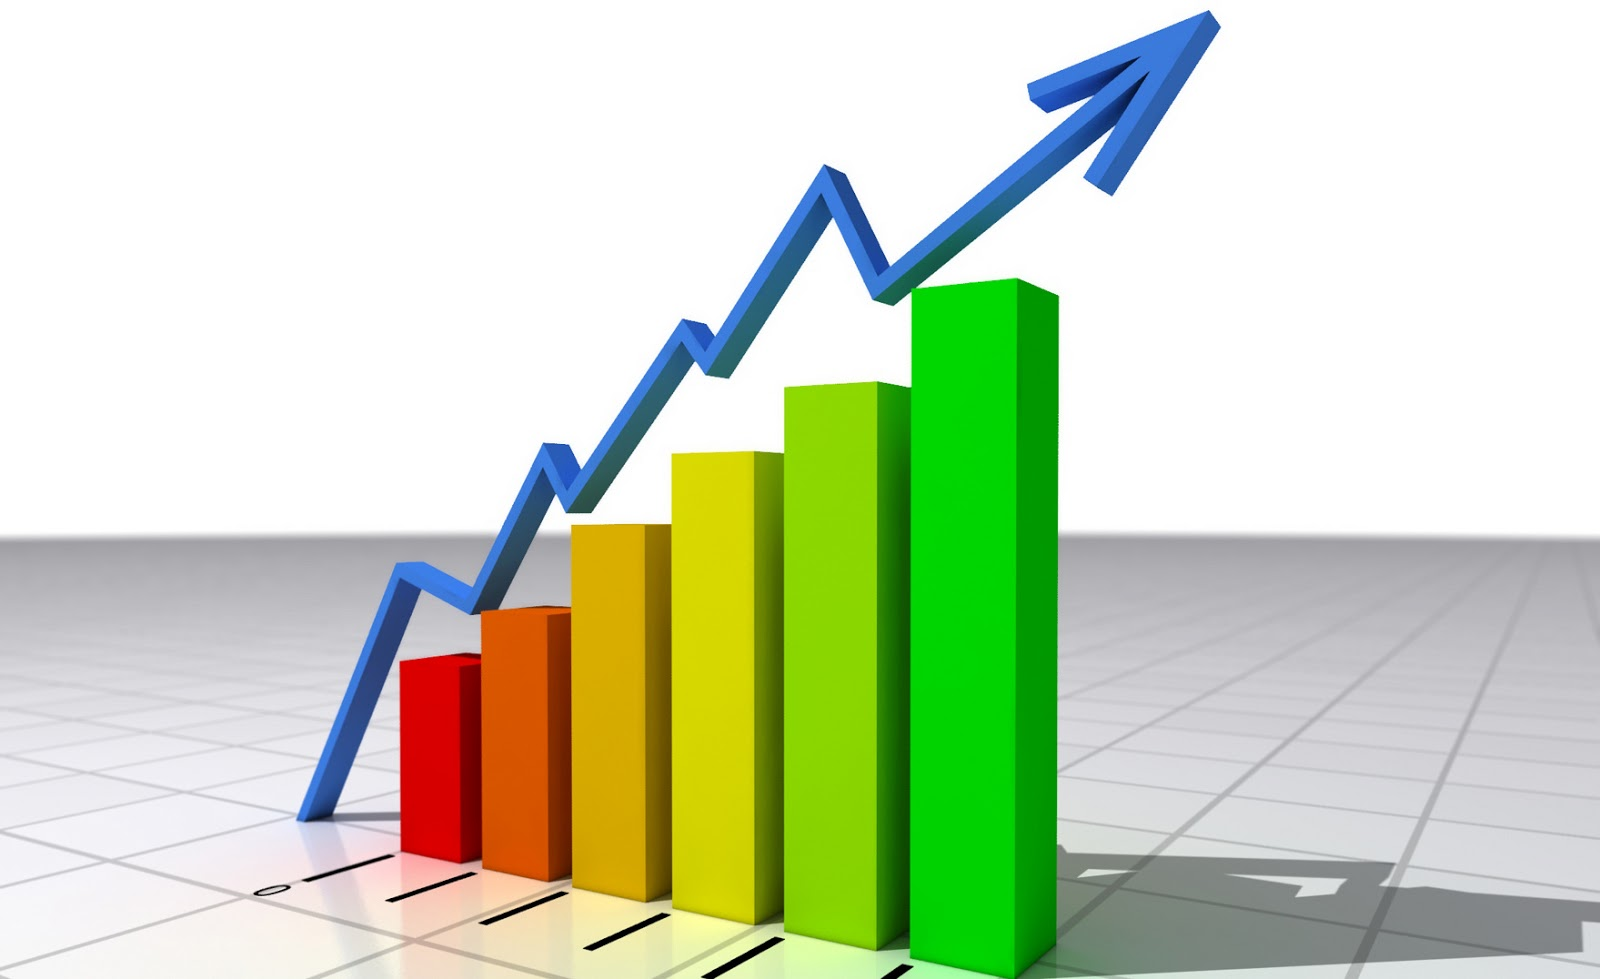
\includegraphics[width=1\linewidth]{ese.jpg}
\end{figure}


%%%%%%%%%%%%%%%%%%%%%%%%%%%%%%%%%%%%%%%%%%%%%%%%%%%%%%%%%%%%%%%%%%%%%%%%%%%%%%%%%%%%%%%%%%%%%%%%%%%%%%%%%%%%%%%%%%
\section{Introducción}
\hyphenation{fun-cio-na-li-dad}
La creación de librerías en lenguajes de programación ayuda a generar una interfaz bien definida para una cierta funcionalidad en específico, 
estas sirven para separar por módulos un programa, y así generar un código más claro y ordenado.\\

Una librería es un conjunto de funciones para desarrollar software, por lo general no son programas, pero si son utilizadas por los programas 
para poder funcionar de forma correcta; el desarrollo de librerías sirve como apoyo para los programadores a tener más facilidades de implementación 
en sus programas y a contar con más recursos para realizar sus proyectos.\\

En este caso, queremos implementar una librería sobre manipulación y análisis de objetos tridimensionales
en el lenguaje C++.\\

La idea  de esta librería es crear métodos o funciones para la manipulación y representación 
de cualquier objeto real, de manera virtual; esta técnica de pasar de un objeto real a representarlo de manera virtual, se utiliza mucho 
en videojuegos, efectos especiales, medicina, simuladores, entre otros.\\

Para nuestro caso utilizaremos para representar los objetos de manera virtual, la técnica de malla de triángulos en 3D, en dónde primero debemos 
representar por medio de una nube de puntos el objeto y luego formar los triangulos con cada uno de esos puntos; para ello utilizaremos el kinect, 
obteniendo así los datos y luego realizar los algoritmos necesarios para la ejecución de las funciones de comparación de datos, generando así la librería.\\


Una segunda parte del proyecto, consiste en la implementación de algunas estructuras de datos para la manipulación de información obtenida mediante el kinect, de manera que se quiere realizar un análisis implementando algunas de ellas, para así determinar y comparar, qué estructuras son las más eficientes a la hora de manipular esta información.\\

En general, las estructuras de datos implementarán las funciones básicas de acceso o búsqueda de datos, lo cual nos ayudará a tener un manejo más rápido y ordenado de los datos obtenidos por el kinect.

ESTA INTRO HAY QUE CAMBIARLAAAAAAAAAAAAAA!!!!!!!!!!!!!!!!!!!!

%%%%%%%%%%%%%%%%%%%%%%%%%%%%%%%%%%%%%%%%%%%%%%%%%%%%%%%%%%%%%%%%%%%%%%%%%%%%%%%%%%%%%%%%%%%%%%%%%%%%%%%%%%%%%%%%%%
\section{Desarrollo}

\subsection{K-Da Library}

Como se mencionó con anterioridad, la creación de librerías de programación corresponden a una funcionalidad en específico. En nuestro caso, la librería
implementada corresponde a un conjunto de métodos computacionales para llevar a cabo la comparación de movimientos. Para lograr esto, se implementó 
la librería en lenguaje C++, sin embargo, los datos de los movimientos son tomados de un controlador de juego libre y entretenimiento llamado Kinect; creado por Alex Kipman, desarrollado por Microsoft para la videoconsola Xbox 360.(http://personales.alumno.upv.es/alrafua/asignaturas/SES/Perifericos/Interfaces\_humanas/camaras\_reconocimiento.html)
Además se usa también el lenguaje de programación Processing para poder obtener del Kinect los datos que se produzcan. Relacionadas estas tres importantes
herramientas es que nuestra librería da el funcionamiento esperado. 

\subsection{Funcionamiento de K-Da Library}

Retomando las herramientas que forman parte de la librería, iniciamos este apartado para describir, de una manera general, como se da la comparación de los movimientos.

\subsubsection{Código en C++}

El código de la librería fue desarrollado en el lenguaje C++. Este código presenta tres diferentes clases, una encargada de recibir los datos de movimiento que provienen del Kinect, sin embargo, es importante mencionar que, en nuestro caso, los movimientos captados son únicamente realizados por humanos, es decir, sí se presenta un movimiento de algún objeto no humano el Kinect no tomará los datos de tal movimiento,
esto ya que está dentro del propio desarrollo del Kinect esta utilizar técnicas de reconocimiento de voz y reconocimiento facial para la identificación automática de los usuarios. (http://malenyabrego.wordpress.com/2011/12/31/mundo-kinect/) Otra de las clases presentes en el código se encarga de convertir los datos (esto último se explicará con mucho más detalle más adelante) que fueron 
recibidos del Kinect y es aquí donde toma participación la última de las clases que es la encargada de realizar la comparación de los movimientos; cabe decir que para realizar una comparación es necesario contar con mínimo dos movimientos.

\subsubsection{Processing}

El lenguaje de programación Processing es la herramienta que utilizamos para tomar los datos que el Kinect genere según el movimiento y convertir estos datos en archivos \textit{.txt} para luego estos, ser utilizados dentro del código en C++. En el código de Processing se pueden elegir 
los movimientos de los que se quieren obtener los datos. Es decir, si necesitamos solo los datos de movimiento que genere el Kinect solo en el \textit{joint} de la muñeca y no de todos los \textit{joints} del diagrama del cuerpo humano en general se puede realizar el cambio dentro del código. En nuestro caso, 
Processing reproduce los datos del movimiento de los \textit{joints} del torso, cuello, hombro y muñeca. 

\subsubsection{Kinect}

Este dispositivo cuenta con una cámara RGB, un sensor de profundidad, un micrófono de múltiples matrices y un procesador personalizado que ejecuta el software patentado, que proporciona captura de movimiento de todo el cuerpo en 3D, reconocimiento facial y capacidades de reconocimiento de voz. 
Son las características anteriores lo que permite que esta última, pero no menos importante, herramienta es la que recolecta los datos del movimiento que se realicen. Utilizando algunos de sus componentes mencionados anteriormente, el Kinect es capaz de grabar los movimientos que realice un humano
frente a él. Los datos que este produce corresponden a puntos de los \textit{joints} en tres dimensiones, largo, ancho y profundidad, o más en general, posiciones en \textit{x}, \textit{y} y \textit{z} de un plano que el mismo Kinect establece. Así bien, durante el movimiento ya sea en el \textit{joint} de la muñeca, hombro o algún otro (según esté especificado en el código Processing), 
el Kinect generará un dato de tres dimensiones para tal \textit{joint} en un tiempo específico, de manera que conforme el movimiento continúa se generan más datos 3D, con diferente posición, y obviamente, en un tiempo diferente. 





%%%%%%%%%%%%%%%%%%%%%%%%%%%%%%%%%%%%%%%%%%%%%%%%%%%%%%%%%%%%%%%%%%%%%%%%%%%%%%%%%%%%%%%%%%%%%%%%%%%%%%%%%%%%%%%%%%
\subsection{Clases}


(Aquí va la explicación de los métodos de Sama y David)\\

Seguidamente los métodos comparar\_angulos y comparar\_velocidad son los que finalmente evalúan que tan bueno estuvo el movimiento y se lo indica al usuario, esto lo hace utilizando como base los datos suministrados por las clases y métodos anteriores. Primeramente el método comparar\_angulos lo que hace es tomar el arreglo de unos y ceros proveniente de arreglo\_promedio y sumar todos los datos del arreglo, al ser este un arreglo de puros unos y ceros y de longitud 10, el valor de esta suma debería ser máximo 10 y mínimo cero, por lo tanto se puede hacer una evaluación de que tan bien estuvo 
el movimiento en base al valor de esta suma, si por ejemplo la suma dió uno, esto quiere decir que solo una decima parte del movimiento lo hizo casi igual o muy parecido al movimiento ``ideal'' por lo tanto el restante 90\% del movimiento lo hizo mal en comparación al movimiento ``ideal'', lo que haría que en general el movimiento haya sido muy malo (para este ejemplo). Si por otro lado la sumatoria dió un valor de 5 esto quiere decir que la mitad del movimiento estuvo bien hecho y la otra mitad no, y así sucesivamente hasta llegar a un valor de la sumatoria de 10, lo cuál significaría evidentemente que el movimiento fue excelente. Seguidamente el método comparar\_velocidad 
lo que hace es determinar que tan rápido el usuario hace el movimiento en comparación con el movimiento ``ideal'', esto ya que de nada serviría tener un 10 en comparar\_angulos si se hizo el movimiento muy lento, ya que efectivamente el movimiento sería igual pero no sería lo correcto decirle al usuario que estuvo bien su movimiento si dura mucho tiempo en ejecutarlo, este método toma la longitud del arreglo de ángulos de los 2 movimientos y los compara, si hay una diferencia de más de un 10\% se lo indica al usuario, diciendole que fue muy lento si se tuvo un 10\% más o que fue muy rápido si se tuvo un 10\% menos. \\
%%%%%%%%%%%%%%%%%%%%%%%%%%%%%%%%%%%%%%%%%%%%%%%%%%%%%%%%%%%%%%%%%%%%%%%%%%%%%%%%%%%%%%%%%%%%%%%%%%%%%%%%%%%%%%%%%%


\section{Referencias}

\begin{enumerate}

\item Richard, J. Computer Science Division. University of California at Berkeley. Triangle. A Two-Dimensional Quality Mesh Generator and 
Delaunay Triangulator. Encontrado el 13 de abril del 2014 en: http://www.cs.cmu.edu/~quake/triangle.html
\item Escenografía Intermedial. Nuevos medios y tecnologías afines a la escena. (15 de mayo del 2012).
Nube de puntos (Point Cloud) con Kinect. Encontrado el 13 de abril del 2014 en: http://escenografiaaumentada.wordpress.com/2012/05/15/148/
\item OPENKINECT. Encontrado el 13 de abril del 2014 en: http://openkinect.org/wiki/Main\_Page
\item Joyanes, L., Sánchez, L. \& Zahonero, I. (2007). Estructuras de datos en C++ (1ra ed.) Madrid: McGraw-Hill / Interamericana de España, S.A.



\end{enumerate}

	
\end{document}

